\section{Extensions of the Basic Model}
The basic model presented in section (\ref{section:derivation:basic_model}) currently has the following limitations
\begin{enumerate}
\item Dynamical systems with complex eigenvalues are ill-defined
\item Only $2d$ of $N$ neurons have nontrivial dynamics. 
\item Network dynamics are inherently periodic and deterministic, not asynchronous. 
\end{enumerate}

We extend the basic model to address these limitations. 

\subsection{Dynamical Systems with Complex Eigenvalues}
\begin{enumerate}


\item Recall the basic self-coupled network equations:

$$
\dot{v}
= 
\begin{bmatrix}
\Lambda & 0
\\
0 & 0
\end{bmatrix}
v +
\begin{bmatrix}
S \left(\Lambda + I_d \right) S & 0
\\
0 & 0
\end{bmatrix}
  \rho 
+ \beta \tilde{c}  
  - 
 \begin{bmatrix}
S^2 & 0
\\
0 & 0
\end{bmatrix}
    \tilde{o},
$$

$$
\dot{\rho} = -\rho + \tilde{o},
$$

$$
\hat{y} = \begin{bmatrix}
S & 0
\end{bmatrix}
\rho.
$$

When the dynamical system $\dot{x} = Ax + Bc$ is oscillatory, the eigenvalues $\Lambda$ of $A=\mathcal{U} \, \Lambda \, \mathcal{U}^T$ are complex, implying $\dot{v}$ is a system of complex equations. Currently, all network quantities are only defined for real-values. Here we generalize the self-coupled network to complex vector space so that it is well defined when $A$ has complex eigenvalues.

The existence of complex eigenvalues implies that $x$ is an element of a complex vector space $\mathbf{C}^d$. The spectral theorem assumes as much when proving the existence of an eigendecomposition for $A = \mathcal{U} \Lambda \mathcal{U}^T$. If we otherwise restrict $x$ to $\mathbf{R}^d$, the eigendecomposition $A$ would exist i.f.f. $A$ was symmetric, i.e. $A = A^T$. 

Complex quantities are often simpler to manipulate in polar coordinates than Cartesian, so we use them here. For any complex scalar $\alpha \in \mathbf{C}$, the relation between polar and Cartesian coordinates is
$$
\alpha = a + i b = \mu e^{i \theta}, 
$$
where
\begin{align*}
\mu &= \sqrt{a^2 + b^2}, 
\\
\\
\theta &= \tan^{-1}\frac{b}{a},
\\
\\
a + ib &= \mu \, cos \,\theta + i \, \mu \,  sin \, \theta = e^{i\theta}.
\end{align*}

\item Let $\bar{\Lambda}$ denote the polar representation of $\Lambda$, the eigenvalues of $A$. 
$$
\bar{\Lambda}_j
\overset{\Delta}{=}
\mu_j \, e^{i \omega_j},
$$

where 

$$
\omega_j = tan^{-1} \frac{\Re\Lambda_j}{\Im\Lambda_j}, 
$$
and
$$
\mu_j = \sqrt{\Re\Lambda_j^2 + \Im\Lambda_j^2}.
$$

$A$'s eigenvalues are
$$
\Lambda = 
\begin{bmatrix}
\Lambda_1 & 0 & \hdots &0  & 0
\\
0 & \Lambda_2 & 0 & \hdots & 0
\\
\vdots & & & & \vdots
\\
 0& 0  & 0 & 0 & \Lambda_d
 \end{bmatrix}
 = 
 \begin{bmatrix}
\mu_1 \, e^{i \omega_1} & 0 & \hdots &0  & 0
\\
0 & \mu_2 \, e^{i \omega_2} & 0 & \hdots & 0
\\
\vdots & & & & \vdots
\\
 0& 0  & 0 & 0 & \mu_d \, e^{i \omega_d}
 \end{bmatrix} = \bar{\Lambda}.
$$

Transforming the eigenvector, we denote the $k^{th}$ complex component of $\mathcal{U}_j$ by $u_{kj}^\Re + i \, u_{kj}^\Im$. Let $W_j$ denote the polar representation of $\mathcal{U}_j$.

$$
\mathcal{U}_j 
=
\begin{bmatrix}
u_{1j}^\Re + i u_{1j}^\Im
\\
\vdots
\\
u_{dj}^\Re + i u_{dj}^\Im
\end{bmatrix}
=
\begin{bmatrix}
\alpha_{1j} e^{i \theta_{1j}}
\\
\vdots
\\
\alpha_{dj} e^{i \theta_{dj}}
\end{bmatrix} = W_j,
$$
where

$$
\alpha_{ij} = \sqrt{(u_{ij}^\Re)^2 + (u_{ij}^\Im)^2},
$$

and

$$
\theta_{ij} = tan^{-1} \frac{u_{ij}^\Im}{u_{ij}^\Re}.
$$


We now write $A$ as 
$$
A = 
W \bar{\Lambda} W^*.
$$

\item The given decoder matrix  $D$ maps integrated spikes from $\mathbf{R}^N$ to the network estimate $\hat{x} \in \mathbf{R}^d$. View $D = \mathcal{U} \begin{bmatrix}S & 0 \end{bmatrix} V^T$ as a sequence of linear maps between vector spaces as in figure (\ref{fig:linear_maps_between_subspaces_D_real}). For complex $\hat{x}$, we require that $D$ map from $\mathbf{C}^N$ to $\mathbf{C}^d$. By assumption, $D$ and $A$ share a common left basis, which is now $W \in \mathbf{C}^{d \times d}$. However the remaining real-valued matrices $S, V$ discard any complex components, limiting the span of $D$ to the complex basis $W$ scaled only by real coefficients, as in figure (\ref{fig:linear_maps_between_subspaces_D_complex}). To ensure that $D$ spans $\mathbf{C}^d$ and not a real-coefficient subspace, we extend $S$ and $V$ to the complex domain. Denote these complexified matrices by $\bar{S}$ and $\bar{V}$ respectively. 

\begin{figure}
\centering
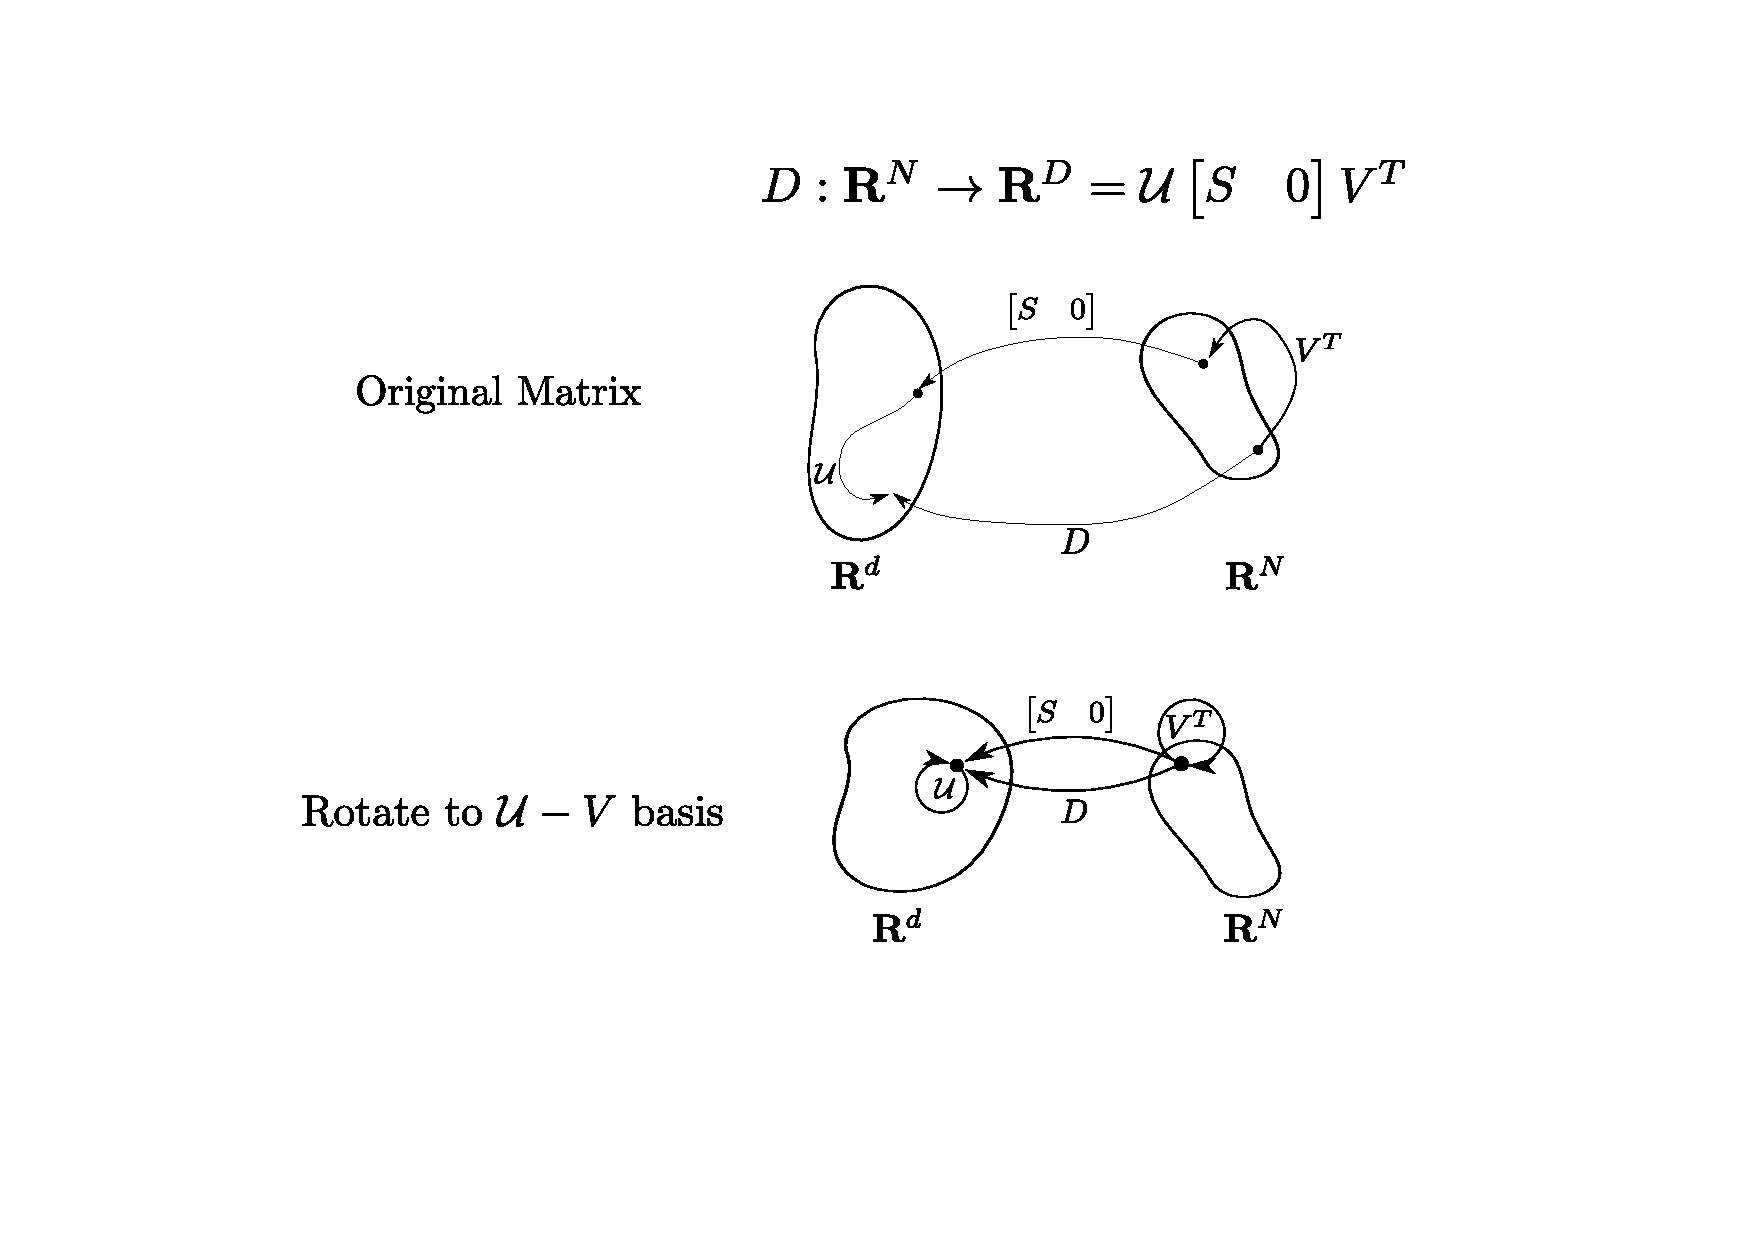
\includegraphics[scale=.6]{figures/linear_map_sequence}
\caption{Visualizing $D$ as a sequence of linear maps between subspaces. \textbf{\textit{Top: }} The matrix $D \in \mathbf{R}^{d \times N}$ is decomposed via SVD into a sequence of 3 linear maps (matrices). The rightmost matrix $V^T \in \mathbf{R}^{N \times N}$ projects a vector  $x$  to give coefficients for the expansion in the basis $V$. The center matrix $\begin{bmatrix} S & 0 \end{bmatrix} \in \mathbf{R}^{d \times N}$ maps vectors from the $V$ basis to a vector in $\mathbf{R}^d$ by scaling and truncation. The leftmost matrix $\mathcal{U} \in \mathbf{R}^{d \times d}$ gives the resultant vector $D x \in \mathbf{R}^d$ by using the scaled vector $\begin{bmatrix} S & 0 \end{bmatrix} V^T$  as coefficients for a basis expansion in $\mathcal{U}$. \textbf{\textit{Bottom:}} We rotate the basis for vectors in $\mathbf{R}^N$ and $\mathbf{R}^d$ to the $\mathcal{U}$ and $V$ bases respectively. This negates the need of $D$ to preemptively project and afterward rotate a vector, leaving only scaling by a diagonal matrix. The mapping $D$ performs on a vector $y$ simplifies to multiplication by a diagonal matrix $S$ of $y$'s first $d$ components. 
}
\label{fig:linear_maps_between_subspaces_D_real}
\end{figure}

\begin{figure}
\centering
\includegraphics[scale=.6]{figures/linear_map_sequence_complex}
\caption{$D$ projects vectors to $\mathbf{R}^d$ before expansion in the basis $W$. \textbf{\textit{Top: }} The matrix $D=W \begin{bmatrix} S & 0 \end{bmatrix} V^T$ shares a complex left-basis $W$ with $A$. However the remaining matrices $S$ and $V$ are real-valued. This limits the range of $D$ to real linear combinations of the basis $W$. \textbf{\textit{Bottom:}} We complexify $S \rightarrow \bar{S}$ and $V \rightarrow \bar{V}$ and rotate network quantities to the $W-\bar{V}$ basis. This ensures that the $span(D) = \mathbf{C}^d$.
}
\label{fig:linear_maps_between_subspaces_D_complex}
\end{figure}

\clearpage

A principled method of extending real functions in $\mathbf{R}^d$ to the complex plane $\mathbf{C}^d$ is to use the Hilbert Transform. Suppose our real function is $f(x)$ and we wish to find $g(x)$ such that $h(x) = f(x) + ig(x)$. The Hilbert transform of $f$ gives a $g$ such that $h$ has at least two useful properties. 1) $h(x)$ is complex-differentiable in $x$; 2) The Fourier transform of $h$ has no negative frequency components, which respects the conjugate-symmetric spectrum of the real-valued $f$. 

Let $H_x(f)$ denote the Hilbert Transform of the function $f$ over the domain $x$, i.e. 

$$
H_x(f) \overset{\Delta}{=} \frac{1}{\pi} \int_{-\infty}^{\infty} \frac{f(y)}{x - y} dy
=
f * \frac{1}{\pi x} (x). 
$$

We complexify the matrix $D$ by applying the Hilbert transform to the columns of $S$ and of $V$ over the domain $k \in \left[ 1,\hdots,d\right]$;  i.e
$$
\bar{S} = 
\begin{bmatrix}
H_k(S_1) & \hdots & H_k(S_d)
\end{bmatrix}  
= H_k(S),
$$

$$
\bar{V} = 
\begin{bmatrix}
H_k(V_1) & \hdots & H_k(V_N)
\end{bmatrix}  
= H_k(V).
$$

Here $k \in \mathbf{Z}$ is a discrete domain of indices, so we use the discrete version of the Hilbert transform.


\item The neurons which implement the network have spike trains $\tilde{o}(\xi) \in \mathbf{C}^{N}$:
    \begin{equation*}
        \tilde{o}_j(\xi) = \sum_{k=1}^{\text{$n_j$ spikes}} \delta(\xi - \xi_{j}^{k}) + i0,
    \end{equation*}
	which have no imaginary component. 
	
    The network's estimate is
	$$
      \hat{y}(\xi) = \begin{bmatrix}
      \bar{S} & 0
      \end{bmatrix} \rho(\xi), 
	$$
    for $\rho = \bar{V}^T r \in \mathbf{C}^N$ where
	$$
        \frac{d\rho}{d \xi} = -\rho + o(\xi).
    $$
	The network error $\epsilon \in \mathbf{C}^d$ is 
	$$
		\epsilon = y - \hat{y}  = W^* e.
	$$


\item Before deriving the network voltage dynamics, we redefine voltage as complex using network optimization. Consider the previous optimization from which voltage was defined
$$
\mathcal{L}(\xi) = || y(\xi + d\xi) - \hat{y}(\xi + d\xi)||^2 = \epsilon^T \epsilon \in \mathbf{R}.$$

The network optimized the Euclidean norm of two real vectors given by the inner product of the error with itself. We generlize to complex vectors by using the complex inner product. I.e, 

$$
\mathcal{L}(\xi) = \epsilon^*\epsilon, 
$$
where $*$ denotes the Hermitian transpose.

When neuron $j$ spikes, the vector $\bar{S}_j$ is added to the network estimate so that the objective is

\begin{align*}
\mathcal{L}_{sp}
&=
(y - \hat{y} - \bar{S}_j)^*(y - \hat{y} - \bar{S}_j)
\\
\\
&=
y^*y - 2 y^*\hat{y} + \hat{y}^*\hat{y} - 2 \bar{S}_j^*(y - \hat{y}) + \bar{S_j}^*\bar{S_j} 
\\
\\
&=
\mathcal{L}_{ns} - 2 \bar{S}_j^*(y - \hat{y}) + \bar{S_j}^*\bar{S_j}.
\end{align*}

We would like to say the spiking condition $\mathcal{L}_{sp} < \mathcal{L}_{ns}$ is then
$$
\bar{S_j}^*\epsilon > \frac{\bar{S}_j^* \bar{S}_j}{2},
$$
however the above equation is between two complex scalars, which have no well-defined ordering. Instead, we take the modulus of either side, which returns a real scalar. This gives the spike condition

$$
|\bar{S}_j^*\epsilon| > \frac{|\bar{S}_j|^2}{2}.
$$
	
This suggests that complex voltage is suitably defined by $\bar{S}_j^*\epsilon$ so that neuron $j$ spikes when 

$$
|v_j| > \frac{\bar{S}_j}{2}.
$$



\clearpage

\item We now derive the voltage dynamics as before. The rotated target dynamical system is

$$
\dot{y} = \bar{\Lambda} y + \beta \tilde{c},
$$

where 
$$
\beta = W^* B W,
$$

$$
\tilde{c} = W^* c.
$$

The error has dynamics

\begin{align*}
\dot{\epsilon} &= \dot{y} - \dot{\hat{y}}
\\
\\
&=
\bar{\Lambda}y + \beta \tilde{c} - \begin{bmatrix}
S & 0
\end{bmatrix}
\dot{\rho}
\\
\\
&= 
\bar{\Lambda}y + \beta \tilde{c}
+
\begin{bmatrix}
S & 0
\end{bmatrix}
\rho
-
\begin{bmatrix}
S & 0
\end{bmatrix}
\tilde{o}.
\end{align*}


Apply the matrix $\begin{bmatrix}
\bar{S} \\ 0
\end{bmatrix}^*$ to both sides to get the voltage dynamics. We write the full set of $N$ equations as
$$
\dot{v} = 
\begin{bmatrix}
\bar{\Lambda} & 0 \\ 0 & 0
\end{bmatrix}
v
+
\begin{bmatrix}
\bar{S}^*\left(I + \bar{\Lambda}\right) \bar{S}  & 0 \\ 0 & 0
\end{bmatrix} \rho 
+
\beta \tilde{c}
-
\begin{bmatrix}
\bar{S}^* \bar{S} &  0 \\ 0 & 0
\end{bmatrix} \tilde{o}.
$$


 
\end{enumerate}

To summarize, the self-coupled network model is extended to complex-valued dynamical systems by the following:
\begin{enumerate}
	\item Factorize $A = \mathcal{U}\Lambda\mathcal{U}^T$, by assumption $\Lambda$ contains complex entries. Rewrite this matrix as $A = W^T \bar{\Lambda} W$ so that $\bar{\Lambda}$ contains only real entries.
	
	\item The voltage contains the sum of real and imaginary components of the error projected onto the rotated (now complex) basis $W$. 
	
	\item 
\end{enumerate}



